\chapter{绪论}
\label{chap:Introduction}
\section{主要研究内容及背景}
%大背景
网络功能虚拟化(Network Function Virtualization,NFV)是由欧洲电信标准组织 (ETSI) 从网络运营商的角度出发提出的一种软件和硬件分离的架构,是当前学术界和工业界十分热门的话题之一。其实质是通过标准化的IT虚拟化技术,采用业界标准的大容量服务器、存储和交换机承载各种各样的网络软件功能,实现软件的灵活加载,从而实现可以在数据中心、网络节点和用户端等不同位置灵活部署。NFV利用标准IT虚拟化技术来加速网络运营商和服务提供商的服务更新,随着近些年来学术界和工业界的携手推进,NFV正在逐步的落地并替代传统的通信服务平台。如今的网络是仍然由各不相同的网络物理设备彼此相连从而实现特定的服务功能,但这样的架构恰恰成为了网络服务更新的掣肘。NFV的目标是使用虚拟的网络功能来替代这些特定的网络设备,在x86等通用性硬件上利用虚拟机化技术来承载大量的网络功能软件,从而降低网络昂贵的设备成本。通过软硬件结构及功能抽象,NFV技术使得网络设备功能不再依赖专用硬件,资源可以充分灵活共享,实现新业务的快速开发,并基于实际业务需求进行自动部署、弹性伸缩、故障隔离和自愈等具体目标 \cite{etsi2013001}。
 
%通用SFC描述
虚拟化资源分配作为NFV管理与编排系统的核心业务一直是工业界和学术界研究的热点问题,而其中的网络功能服务链 (Service Function Chain. SFC) 更是因为其接近实际应用场景的特点,受到众多研究的重点关注 \cite{zave2017dynamic,kulkarni2017nfvnice,mijumbi2016network}。在传统网络中,负载均衡器、网关、虚拟防火墙等网络功能共同被称为业务功能点(Virtual Network Functions, VNFs),而流量在经过了一系列处理后,形成了链式的链式转发拓扑结构即所谓的网络功能服务链。在NFV的应用背景下,各个业务功能点实际上被抽象为软件运行在虚拟化环境(虚拟机或容器)中。与软件定义网络中流量调度方式不同,网络功能服务链的方式更倾向于通过对虚拟网络中各网络功能(虚拟机或容器)的本身进行组合,即以更为灵活的方式实现流量到业务功能点的调配和处理。在网络功能服务链中,网络的转发效率决定了整体网络的性能,而虚拟化资源的分配会影响虚拟网络功能之间实际的通信效率,所以如何优化虚拟化资源分配对于提升NFV性能具有重要意义。

%虚拟化环境中的IMS,IMS中的服务链
在NFV的具体实施中,多媒体子系统 (IP Multimedia Subsystem, IMS) 是较为成熟的一项具体业务,其中更是涌现了众多高质量的达到电信运营级别的开源项目,如Clearwater \cite{clearwater},Kamalio \cite{kamalio}等。在IMS的应用场景下,以Clearwater为例,传统通信的业务与云计算虚拟化技术深度结合,如图 \ref{fig:sample} 所示,各网络功能如代理呼叫会话控制功能(Proxy-Call Session Control Funtion, P-CSCF)、询问和服务会话控制功能(Interrogating\&Serving Session Control Funtion, I/S-CSCF)、SIP服务器(Application Server, AS)等等,以软件的形式运行在特定的虚拟机中,进而由特定功能的虚拟机组成虚拟网络功能的资源池,从而实现网络功能软件化和资源池化的目标。有别于传统的基于专有硬件节点的静态组链(Static Chaining),虚拟化环境中的IMS通过动态地组建网络功能实例形成服务链(Dynamic Chaining) 来提供IMS服务,这样的做的好处是可以依托云计算技术和虚拟化的基础设施,实现服务的快速部署、弹性伸缩。但是,由于IMS业务有其链式服务的特性,各功能节点之间存在逻辑上的链接关系,这对虚拟化基础设施的资源分配提出了新的要求。

首先,传统的虚拟化资源分配以单个虚拟机的为中心,缺乏多个虚拟机协同分配资源的应用场景,从而缺乏相应的资源分配策略。在NFV实际应用场景下,尤其是IMS服务中,服务链的服务形式对虚拟化的资源分配和NFV业务的管理编排需要对协同服务的一组虚拟机进行操作,在考虑到物理资源数量的同时也要考虑资源本身的亲和度关系,这样的资源分配方式对现有的虚拟化资源管理平台提出了全新的挑战。其次,当前市场上广泛使用的大通量服务器 (Commodity Server) 大多为多核的非一致性存储访问架构架构(Non-Uniform Memory Access, NUMA)。这种架构本身具有异构的特点,不同的物理资源之间的亲和度具有较大的差异,而现有的虚拟化平台缺乏有效的手段将此类信息传递给已有的资源分配算法\cite{},从而导致其失去优化效果。
\begin{figure}[!htp]
	\centering
	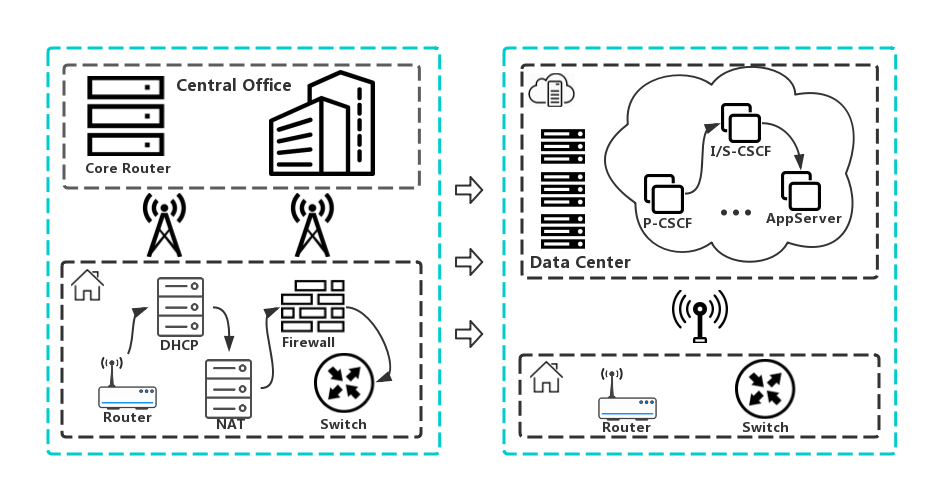
\includegraphics[width=0.8\textwidth]{sample.png}
	\bicaption[fig:sample]{云环境中的IMS服务}{云环境中的IMS服务}{Fig}{IMS in Cloud}
\end{figure}
		
学术界目前对于NFV研究主要集中在两方面:(1)优化通用操作系统和网络协议栈,自底向上地提升NFV应用的性能,打破网络服务中来自底层通用平台和通用操作系统的性能瓶颈。(2)提出针对NFV应用的资源分配算法,优化网络功能服务节点间网络流量的实际路径。其中,在优化通用操作系统网络协议栈的方向,近些年学术界涌现了一系列的研究 \cite{rizzo2012netmap,ram2013hyper,belay2014ix,hwang2015netvm,yasukata2016stackmap,prekas2017zygos},结合工业界提出的高速网络包转发框架DPDK \cite{intel2015data} ,从简化网络协议栈,重新分配虚拟化资源和减少无关开销等角度优化基于通用服务器的操作系统和虚拟化框架。这些方法都提高了标准通用服务器的在NFV场景下的网络性能,然而仅仅做到网络转发性能的提升是不够的,这些研究并未对实际的NFV应用进行针对性的优化,忽略了NFV应用的特有的各网络功能节点间如服务链这样的组织形式,仍然从一般系统软件的角度去提升基础网络性能,缺乏对NFV应用组织结构的认识和建模。文献 \citen{xie2016service} 指出在NFV资源分配问题 (NFV resource allocation,NFV-RA) 中,如何解决基于NFV网络基础设施的资源分配是一项重要的挑战。进一步的,文献 \citen{herrera2016resource} 中将该问题划分为更细的粒度进行深入研究,为研究此类的问题提供了具体的研究方向。NFV网络基础设施的资源分配问题与文献 \citen{belbekkouche2012resource,fischer2013virtual} 所提出的传统网络中的网络功能映射问题 (Virtual Network Embedding,VNE) 相关,已有的研究参照VNE问题的研究成果和NFV背景下的具体问题,提出了一系列与实际应用相结合的算法来尝试解决在NFV场景中资源分配问题。其中,有的从网络时延角度出发,如文献 \citen{mijumbi2015design} 所述,对NFV的部署和映射问题进行建模,给出了基于贪心和禁忌搜索的两种针对虚拟网络功能转发图映射和虚拟网络功能调度子问题的求解。文献 \citen{lin2016demand} 从网络开销角度出发,提出了基于混合整数线性规划的方法来最小化网络功能的部署和网络流量的路由问题。这些研究都从资源分配角度结合NFV的应用特点给出了解决问题的思路,但是大部分研究使用仿真的平台进行算法有效性的验证,对于求解问题实际物理平台上的可行性缺乏有力的证明。

%TODO 全文总结
本文着眼于实际的IMS平台,利用已经实现的NFV应用来验证在大容量通用服务器中未对服务链进行有效优化的资源分配存在的挑战,对这一实际问题进行了重新建模,基于多核物理机的非一致性存储访问特性 (NUMA) 提出了优化解决方案,并在Clearwater平台上实现了原型系统,通过修改Clearwater的动态服务链映射策略实现了基于服务链和底层资源的映射方法。实验证明,经过本系统的优化过后,Clearwater服务的性能得到了有效的提升。


\section{国内外研究现状}
\label{intro:research}
本节介绍并讨论与研究课题相关的国内外研究现状与发展趋势,重点包括国内外研究中对网络功能虚拟化中服务链问题的介绍,针对网络I/O优化,NFV资源分配问题,以及国内外研究者在多核架构下针对该问题的一些研究成果。同时,本章中也将本文所设计的优化解决方案与已有的解决方案和处理思路进行对比,对相关研究的研究内容进行比较和优缺点的分析。

\subsection{网络功能服务链}
根据文献 \citen{bhamare2016survey} 的定义,网络功能服务链是抽象服务功能 (Service Function,SF) 的有序或部分有序集合,包括对数据包,数据帧和数据流的有序约束分组。在实际的NFV场景下,由于服务拓扑的复杂性,各个功能节点在服务链中的位置应具有相对的灵活性。对于NFV中SFC的研究方兴未艾,文献 \citen{quinn2015problem} 总结了现阶段SFC研究所面临的挑战,主要包括:(1)复杂的网络拓扑依赖。原有的服务链是在硬件层面实现的,网络功能与底层硬件拓扑是绑定的,因此网络功能的增加与删减需要直接操作硬件,而NFV所带来的虚拟网络功能需要网络管理员最大可能的优化利用现有的网络资源,复杂的网络拓扑会给动态管理网络功能带来挑战。(2)严格的配置管理。服务链的网络功能节点顺序有着严格的要求,错误的服务配置会导致服务失败,严重影响服务质量,因此如何保证服务链的正确配置也是业界重点关注的领域。(3)受约束的服务弹性。服务链复杂的拓扑限制了服务链快速伸缩的弹性,服务链中任何一个网络节点的失效都可能导致服务链的伸缩失败,保证服务链所以功能节点的可用性对实现可扩展的服务链具有重要意义。文献 \citen{ghaznavi2015elastic} 研究了在弹性网络功能下的服务链放置问题,虽然与传统的网络放置问题相似,但网络功能额外的灵活有序要求对该类问题进行重新建模,并基于新的模型进行求解和优化。本文所研究的网络功能服务链是基于传统的串行服务链,针对服务链所运行的通用服务器平台资源进行建模并优化求解。相比于已有的研究,本文使用更接近实际应用平台的具体NFV业务,并借助虚拟化平台和具体业务平台来具体实现NFV业务,可以使用真实的应用场景和平台来验证本文所提出系统的有效性。

\subsection{网络I/O优化}
为了减小在虚拟化环境中运行虚拟机所带来的额外开销,文献 \citen{martins2014clickos} 对虚拟机操作系统进行了裁剪,使用微内核的方式构建了基于MiniOS \cite{popuri2014tour} 的最小化操作系统ClickOS,并在Xen \cite{barham2003xen} 的基础上将后端交换机Open vSwith \cite{pfaff2015design} 替换为了高速的VALE交换机 \cite{rizzo2012netmap} ,使用Click语言 \cite{kohler2000click} 进行NFV网络功能逻辑搭建,从而大大减少了虚拟化所带来的性能开销,提升了虚拟机的网络吞吐。但是在小包的测试环境中,该系统出现了剧烈的性能抖动,而且所能实现虚拟网络功能仍处于单个功能节点阶段,尚未组成服务链,并不能满足NFV复杂的业务需求。相比文献 \citen{martins2014clickos} ,文献 \citen{hwang2015netvm} 基于KVM平台 \cite{kivity2007kvm} 推出了NetVM,利用了高速的包转发框架DPDK \cite{intel2015data} 大大提升了网络协议栈的包转发速率,并通过共享大页内存、零拷贝数据传输以及优化CPU调度器提升了数据在VM之间的传输效率,减少了由于虚拟化中虚拟CPU的调度所引起的上下文切换开销。本文中借鉴了文献 \citen{hwang2015netvm} 的平台,在KVM基础上使用virtio \cite{russell2008virtio} 方式来优化VM之间的网络传输性能,通过优化多核服务器中虚拟机间资源的亲和度关系,解决在SFC的背景下NFV应用的性能优化问题。

文献 \citen{panda2016netbricks} 针对基于虚拟化技术实现的NFV提出不同的看法,认为基于现有的虚拟化技术 (VM或容器)所提供的隔离性会带来很高的性能开销,并且针对虚拟化来开发相应的网络功能是个十分繁琐的过程,为了减少这类与服务无关的开销,他们提出了一个新的NFV框架NetBricks来解决这两个问题。对于构建NF,文献 \citen{panda2016netbricks} 使用Rust语言构建了一小组可定制的网络处理元素,利用该语言的类型检查和安全运行机制来提供基于软件的隔离,将网络功能虚拟化与虚拟化框架解耦,使得软件化的网络功能不再依赖虚拟化平台,极大地减少了构建网络功能的开销,从而实现整体I/O性能的提升。文献 \citen{panda2016netbricks} 所提出的优化思路十分值得借鉴,但是现阶段完全抛开虚拟化框架实现NFV的成本太高,而且现有的虚拟化管理框架所带来的优势并不能体现,这样的做法会使得NFV失去与当前云计算平台相结合的优势。本文依然采用的是基于KVM的虚拟机实现模式,尽管虚拟化会引起较高的开销,但是同时所带来的更加简单的实现方式,以及更好的隔离性保障可以使得本设计专注于解决服务链的资源分配问题。


\subsection{NFV资源分配问题}
在NFV资源分配问题方面,文献 \citen{herrera2016resource} 详细介绍了NFV资源分配问题的研究现状,总结了资源分配问题的具体子问题,即虚拟网络功能组链 (VNFs Chain Composition,VNFs-CC), 网络转发图映射 (VNF-Forwarding Graph Embedding,VNF-FGE)和虚拟网络功能调度 (VNFs Scheduling, VNFs-SCH)。文献 \citen{herrera2016resource} 将NFV下的资源分配问题归结为一类NP-Hard问题,并指出了解决此类问题的三种解法思路:确定解法、启发式解法和元启发式解法。具体来讲,针对VNF-FGE问题,确定解法中的整数线性规划方法可以在可接受的时间内给出最优解。而在时间敏感的NFV资源分配问题下,确定解法的时间开销超出了预期限制,这时就需要借助基于启发式和元启发式的高级算法来减少算法的运行时间和额外开销。根据文献 \citen{herrera2016resource} 的归纳和总结,本文沿用了其解决该类问题的解法思路,使用基于整数线性规划的确定解法来解决较小规模下的虚拟网络功能组链和映射问题。

文献 \citen{hsieh2016network} 认为在数据中心,网路功能服务链使工作流以特定的顺序遍历不同的网络功能,为客户提供不同级别的服务。由于服务链中任何相邻网络功能之间的距离将决定该链路的总带宽消耗,那么虚拟化网络功能在数据中心中的放置便成为了影响整体带宽的重要问题。在文献 \citen{hsieh2016network} 中,这种放置问题被归结为一个多重背包问题 (Multiple Knapsack Problem) 。文献 \citen{hsieh2016network} 针对树状网络拓扑,文章提出了两种基于贪心的算法:多层最差拟合和多层最佳拟合。在仿真平台的实验结果表明,与传统的最优算法相比,优化算法可以将带宽消耗降低15\%,而使用服务器数量仅增加1\%。文献 \citen{hsieh2016network} 使用组合优化的思想来归结此类问题可以使得问题变得更加清晰明了,但是算法仅在仿真平台上得到了验证,本文则利用真实的NFV应用平台对所提出的算法进行了验证。


\subsection{其他相关研究}
除了对于网络I/O的优化和NFV资源分配问题的研究,很多文献和论文也从其他角度如MANO系统和操作系统线程等方面,对网络功能虚拟化进行了研究。

文献 \citen{mijumbi2016management} 总结了在网络功能虚拟化管理和编排时可能会遇到的挑战。文章结合虚拟化所带来的资源体量的增加,分析了如何在现有的庞大的基础设施中获取有效的产出所需要面对三个主要问题:(1) NFV服务点 (Points of Presence, PoP) 的地理分布,为了更好地服务用户,如何确定虚拟网络功能集群的服务点地里位置对于电信运营商来说是重点挑战之一。严格的服务质量要求按照一定的最优化问题的方法来合理部署NFV服务的存在点,从而使得NFV服务可以保证覆盖所有服务范围。(2)虚拟网络功能放置,网络功能虚拟化是以一定逻辑链接的虚拟网络功能所组成的,服务链就是一种典型的组成形式,在NFV服务点中如何去合理部署具体的虚拟网络功能对于MANO框架来说具有重要意义。(3)动态资源管理,NFV服务的弹性需求要求MANO系统同样能够支持动态地分配和调度物理资源以实现服务链的伸缩目标,能够满足不同需求规模下的服务实现。

文献 \citen{hu2016towards} 从NFV具体部署的大通量标准服务器出发,认为在实际运行时会面临许多挑战。因为NFV数据平面及其服务功能链的复杂性特征,现代NFV应用以异构软件流水线的方式部署在大容量通用服务器上。文献 \citen{hu2016towards} 从操作系统运行线程的角度出发,考虑到NFV应用流量必须由异构处理软件从网卡到终端接收器。由于流程的端到端性能是由每个处理阶段的性能共同决定的,基于底层物理架构的的大容量通用服务器中的资源分配映射方案必须考虑线程间的依赖调度来减少资源竞争所带来的影响。因此,在文献 \citen{hu2016towards} 中,他们提出了一个可以协同放置最小化端到端访问开销的线程调度机制来最小化NFV线程应用线程端到端的数据传递开销。为了更加方便地评估各线程的数据传递开销,文献 \citen{hu2016towards} 还提出了一个基于线程资源的NFV应用性能下降模型,通过这个模型来衡量数据异构的软件流水线中传递时所造成的开销。本文相比于文献 \citen{hu2016towards},更加侧重于考虑虚拟化的资源分配所造成的影响,虽然从主机的角度来看,虚拟机也是以线程方式运行在主机上,但是虚拟机软件栈会屏蔽虚拟机内部应用的具体信息,而且现有虚拟机的I/O虚拟化技术也会对虚拟机线程间的数据传递有重要影响,本文结合virtio的I/O虚拟化方式,从虚拟机的角度来解决NFV应用的资源分配问题,从而提高NFV应用的整体性能。

\section{论文安排}
本文对网络功能虚拟化中,虚拟机资源调度进行了研究,论文的具体结构和内容安排如下:

第一章作为绪论,主要介绍了本课题的主要研究内容和研究背景。进一步的对于本研究相关的工作进行了介绍和梳理,主要从网络I/O优化研究和NFV资源分配研究两个角度以及其他相关研究介绍了国内外已有的研究成果。最后本章对全文的结构和安排做了介绍。

第二章重点介绍了与本文的研究紧密相关的研究背景和相关技术,包括NFV的发展历程,本文所使用的NFV应用平台Clearwater,目前主流的网络I/O虚拟化技术分类,多核服务器非一致性存储访问架构,最后还介绍了在多核服务器下的虚拟机性能观测实验,为读者了解与研究相关的知识和下文的展开做了准备。

%TODO:记得修改
第三章着重介绍了本文中研究方案的具体设计,包括方案的设计目标,基于服务链的建模,系统的设计思路和系统具体的模块设计等。同时,也依次详细介绍了文本的设计方案的各个子模块的具体设计思路,描述了基于模块设计的系统工作流。

第四章将介绍本研究中的研究方案的具体实现,以总体算法框架为切入点,分模块介绍了本文系统各子模块的实现方法。

第五章从实验的角度对本文的设计进行了性能上的测试。通过利用Clearwater自带的压力测试工具和基础性能测试工具iPerf、Ping、Apache等,在真实的测试环境下对本文所提出的系统进行了严格的测试。

第六章归纳全文,总结和回顾了全文的研究内容和主要研究结论,并提出了一些研究展望。

\section{本章小结}
本章主要整理和归纳与本研究密切相关的国内外研究现状和发展趋势。本章中,重点介绍了国内外的相关研究中,网络功能虚拟化带来的一系列挑战和存在的问题。同时,本章中也对现有解决方案进行了深入的探讨,分析这些方案的共同点和优缺点,与本研究中的设计相对比。本章也对网络功能虚拟化的研究热点进行了介绍,特别是对当前研究较为火热的资源调度问题及相关研究的研究成果进行了简单的归纳和总结。